\chapter{\uppercase{Circuits elèctrics i electrònics}}
\section{Circuits electrònics amb CircuiTikz}
Alguns exemples de circuits.

\begin{center}
\begin{circuitikz} \draw
(0,0) to[ variable cute inductor ] (2,0); 
\end{circuitikz}
\end{center}

\begin{center}
\begin{circuitikz}[american voltages]
\draw
  (0,0) to [short, *-] (6,0)
  to [V, l_=$\mathrm{j}{\omega}_m \underline{\psi}^s_R$] (6,2) 
  to [R, l_=$R_R$] (6,4) 
  to [short, i_=$\underline{i}^s_R$] (5,4) 
  (0,0) to [open, v^>=$\underline{u}^s_s$] (0,4) 
  to [short, *- ,i=$\underline{i}^s_s$] (1,4) 
  to [R, l=$R_s$] (3,4)
  to [L, l=$L_{\sigma}$] (5,4) 
  to [short, i_=$\underline{i}^s_M$] (5,3) 
  to [L, l_=$L_M$] (5,0); 
\end{circuitikz}
\end{center}


\subsection{Títol de la subsecció}

\begin{center}

\begin{tikzpicture}
    \draw
    % Thyristors leg 2
    (1.5,0)
        to[Ty] ++(0,1.5)
        -- ++(0,1)
        to[Ty] ++(0,1.5) coordinate (leg2)
    % Thyristors leg 1
    (0,0)
        to[Ty] ++(0,1.5)
        -- ++(0,1)
        to[Ty] ++(0,1.5) coordinate (leg1)
    % Connections and load RL
        -- ++(2,0)
        to[short, i=$i_o$, current/distance=0.5] ++(2,0)
        -- ++(0,-0.8)
        to[R] ++(0,-1.2)
        to[L] ++(0,-1.2)
    % Back to (0,0)
        |- (0,0)
    % AC source
    (-2,1.5) coordinate (Vnn)
        to[sV] ++(0,1) coordinate (Vpp)
        -- (leg1 |- Vpp) node [circ] {}
    (Vnn)
        -- (leg2 |- Vnn) node [circ] {}
    % v_o(t)
    (4.5,3.5)
        to[open, v^=$v_o(t)$] ++(0,-3)
    ;
\end{tikzpicture}

\bigskip

\begin{tikzpicture}[scale=0.85]
    \draw
(0,0) to [battery, invert, , v<=$U_q$] (0,4)
	to[ammeter, f=$i_1$] (4,4)
	to[R=, l=$R_1$,a=1\si{\kohm}] (4,2) %l=1 \si{\kohm}, v=2\si{\kohm}
	to[C=$C_1$] (4,0) -- (3.5,0)
	to[lamp, *-*] (0.5, 0) -- (0,0)
(0.5,0) -- (0.5,-2)
	to[voltmeter, color=red] (3.5, -2) -- (3.5,0)
    ;
\end{tikzpicture}

\vspace{10pt}
\vspace{1cm}
\bigskip
\bigskip
Per tenir la fletxa del corrent coincident amb el cable, i. Per fora el cable, f.
\begin{figure}
\centering
\begin{tikzpicture}[scale=0.85]
    \draw
    (4,2) node[nigfete,] (fet) {} %rotate=90
    
(0,0) to [battery, invert, , v<=$V_E$] (0,4)
	to[L, l=$L_1$, i=$i_L$] (4,4) %i per intensitat, f per flow
(fet.D) to [short, f<=$i_T$] (4,4)
	(fet.S) to (4,0) -- (0,0) %l=1 \si{\kohm}, v=2\si{\kohm} 
(4,4) to [D*, l=$D_1$, f>^=$i_D$] (7,4)
	to [C, l=$C_1$, f>^=$i_C$] (7,0) -- (4,0)
(7,4) -- (9,4) node[label={[font=\footnotesize]above:$V_O$}] {}
 to [R, *-*, l=$R_{load}$, f>^=$i_R$] (9,0) -- (6,0)
(0,0) -- node[ground, scale=1.5] {} (0,-0.1)
    ;
\end{tikzpicture}
\caption{M1} \label{fig:M1}
\end{figure}

\bigskip
\bigskip
\end{center}
Abans hem mostrat un convertidor Boost \ref{fig:M1}.\\
Una gràfica, treta d'Internet. Molt elegant, però a hores d'ara em sento més còmode amb Python i matplotlib.\\
\begin{center}
% Example 4-7, p. 135 of Hart, discontinuous current in full-wave rect
\begin{tikzpicture}
\begin{scope}[xscale=1,yscale=1.5]
    \newcommand{\alphaa}{60 * pi / 180}
    \newcommand{\betaa}{216 * pi / 180}

    \draw[thin, ->] (-0.2, 0) -- (14,0) node[right] {$\omega t$};

    \foreach \x/\xtext in {0,{\alphaa}/\alpha,{pi}/\pi,
      {\betaa}/~,{2*pi}/{2\pi},{3*pi}/{3\pi}}
        \draw (\x,0.1) -- (\x,-0.1) node [below] {$\xtext$};
    \draw (\betaa,-0.1) -- (\betaa,0.1) node [above] {$\beta$};


    % Vs
    \draw[domain=0:14, help lines, smooth]
        plot (\x,{sin(\x r)});
    % -Vs
    \draw[domain=0:14, help lines, smooth]
        plot (\x,{-sin(\x r)});
    % Vo and Io
    \foreach \qq [evaluate=\qq as \qqshft using \qq*pi] in {0,...,3}
    {
    \begin{scope}[xshift=\qqshft cm,
        every path/.style={ultra thick, color=red}]
        % Vo
         \draw[domain=0:{\betaa-pi}]
             plot (\x,{-sin(\x r)})
             -- ({\betaa-pi},0)
             -| (\alphaa,{sin(\alphaa r)})
         [domain=\alphaa:pi]
             plot (\x,{sin(\x r)});
         % Io
         \draw
         [domain=\alphaa:\betaa,color=blue,thick]
             plot (\x,{0.05 * (13.6*sin((\x - 0.646)*180/pi)
               - 21.2*exp(-\x/0.754))});
    \end{scope}
    }
    \node[right,color=red] at ({pi/2+pi/12},1.05) {$v_o$};
    \node[right,color=blue] at ({pi/2+pi/3},0.8) {$i_o$};
\end{scope}
\end{tikzpicture}

\end{center} %si aquí fes un intro, queda el tab, cosa que en principi no m'interessa.
Per inserir codi podeu inserir-lo dintre les etiquetes \verb|lstlisting*| que he configurat al main. Canvieu-lo si el codi no és Python, que és el que hi ha per defecte.

%insereix el codi aquí sota
\begin{lstlisting}
import matplotlib.pyplot as plt
# use LaTeX fonts in the plot
plt.rc('text', usetex=True)
plt.rc('font', family='serif')
# get the figure
f = plt.figure()


inicial = 5000
interes = 0.15

x = [1,2,3,4,5,6,7,8,9,10,11,12,13,14,15,16,17,18,19,20]
y = [1,2,3,4,5,6,7,8,9,10,11,12,13,14,15,16,17,18,19,20]
for i in range(15):
    y[i]=inicial*pow((1+interes), x[i])


# set labels (LaTeX can be used)
plt.title(r'\textbf{Mutual Information Feature Selection}', fontsize=11)
plt.xlabel(r'\textbf{Best K features}', fontsize=11)
plt.ylabel(r'\textbf{AUC Score on split11 Dataset}', fontsize=11)

plt.plot(x,y, label='Exponential')
plt.legend(loc='upper left')
# plt.grid()
plt.show()

# save as PDF
f.savefig("fs_mi.pdf", bbox_inches='tight')
\end{lstlisting}

\begin{center}
  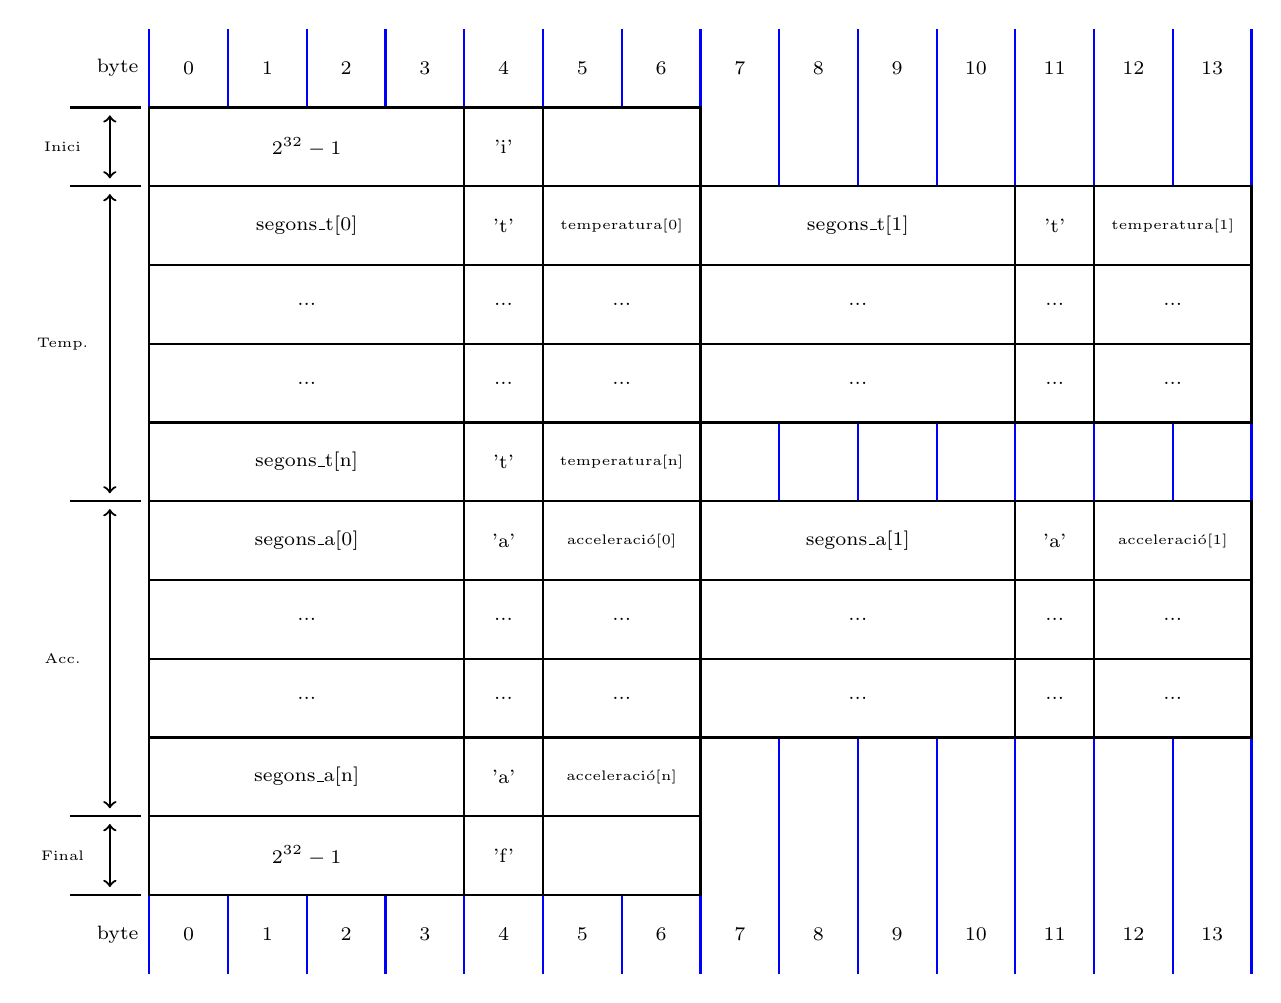
\begin{tikzpicture}[scale=1]
	\foreach \x in {0,...,13}
		\node at (\x+0.5,20.5) {\scriptsize \x};
	\foreach \x in {0,...,13}
		\node at (\x+0.5,9.5) {\scriptsize \x};
	\foreach \x in {0,...,14}
		\draw[thick, blue] (\x,9) -- (\x,21);
	\node[thick] (bit1) at (-0.4,20.5) {\scriptsize byte};
	\node[thick] (bit2) at (-0.4,9.5) {\scriptsize byte};
	\draw [<->, thick] (-0.5, 18.9) -- (-0.5,15.1);
	\draw [<->, thick] (-0.5, 19.9) -- (-0.5,19.1);
	\draw [<->, thick] (-0.5, 14.9) -- (-0.5,11.1);
	\draw [<->, thick] (-0.5, 10.9) -- (-0.5,10.1);
	\draw [thick] (-1, 20) -- (-0.1,20);
	\draw [thick] (-1, 19) -- (-0.1,19);
	\draw [thick] (-1, 15) -- (-0.1,15);
	\draw [thick] (-1, 11) -- (-0.1,11);
	\draw [thick] (-1, 10) -- (-0.1,10);
	\node[fill=white] at (-1.1,19.5) {\tiny Inici};
	\node[fill=white] at (-1.1,17) {\tiny Temp.};
	\node[fill=white] at (-1.1,13) {\tiny Acc.};
	\node[fill=white] at (-1.1,10.5) {\tiny Final};

	\filldraw[thick,draw=black, fill=white] (0,20) rectangle (4,19); \node (mode) at (2,19.5) {\scriptsize $2^{32}-1$};
	\filldraw[thick,draw=black, fill=white] (4,20) rectangle (5,19); \node (mode) at (4.5,19.5) {\scriptsize 'i'};
	\filldraw[thick,draw=black, fill=white] (5,20) rectangle (7,19); \node (mode) at (6,19.5) {\scriptsize };

	\filldraw[thick,draw=black, fill=white] (0,19) rectangle (4,18); \node (mode) at (2,18.5) {\scriptsize segons\_t[0]};
	\filldraw[thick,draw=black, fill=white] (4,19) rectangle (5,18); \node (mode) at (4.5,18.5) {\scriptsize 't'};
	\filldraw[thick,draw=black, fill=white] (5,19) rectangle (7,18); \node (mode) at (6,18.5) {\tiny {temperatura[0]}};
    \filldraw[thick,draw=black, fill=white] (7,19) rectangle (11,18); \node (mode) at (9,18.5) {\scriptsize segons\_t[1]};
	\filldraw[thick,draw=black, fill=white] (11,19) rectangle (12,18); \node (mode) at (11.5,18.5) {\scriptsize 't'};
	\filldraw[thick,draw=black, fill=white] (12,19) rectangle (14,18); \node (mode) at (13,18.5) {\tiny temperatura[1]};
	
	
	\filldraw[thick,draw=black, fill=white] (0,18) rectangle (4,17); \node (mode) at (2,17.5) {\scriptsize ...};
	\filldraw[thick,draw=black, fill=white] (4,18) rectangle (5,17); \node (mode) at (4.5,17.5) {\scriptsize ...};
	\filldraw[thick,draw=black, fill=white] (5,18) rectangle (7,17); \node (mode) at (6,17.5) {\scriptsize ...};
    \filldraw[thick,draw=black, fill=white] (7,18) rectangle (11,17); \node (mode) at (9,17.5) {\scriptsize ...};
	\filldraw[thick,draw=black, fill=white] (11,18) rectangle (12,17); \node (mode) at (11.5,17.5) {\scriptsize ...};
	\filldraw[thick,draw=black, fill=white] (12,18) rectangle (14,17); \node (mode) at (13,17.5) {\scriptsize ...};
	
	\filldraw[thick,draw=black, fill=white] (0,17) rectangle (4,16); \node (mode) at (2,16.5) {\scriptsize ...};
	\filldraw[thick,draw=black, fill=white] (4,17) rectangle (5,16); \node (mode) at (4.5,16.5) {\scriptsize ...};
	\filldraw[thick,draw=black, fill=white] (5,17) rectangle (7,16); \node (mode) at (6,16.5) {\scriptsize ...};
    \filldraw[thick,draw=black, fill=white] (7,17) rectangle (11,16); \node (mode) at (9,16.5) {\scriptsize ...};
	\filldraw[thick,draw=black, fill=white] (11,17) rectangle (12,16); \node (mode) at (11.5,16.5) {\scriptsize ...};
	\filldraw[thick,draw=black, fill=white] (12,17) rectangle (14,16); \node (mode) at (13,16.5) {\scriptsize ...};
	
	\filldraw[thick,draw=black, fill=white] (0,16) rectangle (4,15); \node (mode) at (2,15.5) {\scriptsize segons\_t[n]};
	\filldraw[thick,draw=black, fill=white] (4,16) rectangle (5,15); \node (mode) at (4.5,15.5) {\scriptsize 't'};
	\filldraw[thick,draw=black, fill=white] (5,16) rectangle (7,15); \node (mode) at (6,15.5) {\tiny temperatura[n]};



	\filldraw[thick,draw=black, fill=white] (0,15) rectangle (4,14); \node (mode) at (2,14.5) {\scriptsize segons\_a[0]};
	\filldraw[thick,draw=black, fill=white] (4,15) rectangle (5,14); \node (mode) at (4.5,14.5) {\scriptsize 'a'};
	\filldraw[thick,draw=black, fill=white] (5,15) rectangle (7,14); \node (mode) at (6,14.5) {\tiny acceleració[0]};
    \filldraw[thick,draw=black, fill=white] (7,15) rectangle (11,14); \node (mode) at (9,14.5) {\scriptsize segons\_a[1]};
	\filldraw[thick,draw=black, fill=white] (11,15) rectangle (12,14); \node (mode) at (11.5,14.5) {\scriptsize 'a'};
	\filldraw[thick,draw=black, fill=white] (12,15) rectangle (14,14); \node (mode) at (13,14.5) {\tiny acceleració[1]};
	
	
	\filldraw[thick,draw=black, fill=white] (0,14) rectangle (4,13); \node (mode) at (2,13.5) {\scriptsize ...};
	\filldraw[thick,draw=black, fill=white] (4,14) rectangle (5,13); \node (mode) at (4.5,13.5) {\scriptsize ...};
	\filldraw[thick,draw=black, fill=white] (5,14) rectangle (7,13); \node (mode) at (6,13.5) {\scriptsize ...};
    \filldraw[thick,draw=black, fill=white] (7,14) rectangle (11,13); \node (mode) at (9,13.5) {\scriptsize ...};
	\filldraw[thick,draw=black, fill=white] (11,14) rectangle (12,13); \node (mode) at (11.5,13.5) {\scriptsize ...};
	\filldraw[thick,draw=black, fill=white] (12,14) rectangle (14,13); \node (mode) at (13,13.5) {\scriptsize ...};
	
	\filldraw[thick,draw=black, fill=white] (0,13) rectangle (4,12); \node (mode) at (2,12.5) {\scriptsize ...};
	\filldraw[thick,draw=black, fill=white] (4,13) rectangle (5,12); \node (mode) at (4.5,12.5) {\scriptsize ...};
	\filldraw[thick,draw=black, fill=white] (5,13) rectangle (7,12); \node (mode) at (6,12.5) {\scriptsize ...};
    \filldraw[thick,draw=black, fill=white] (7,13) rectangle (11,12); \node (mode) at (9,12.5) {\scriptsize ...};
	\filldraw[thick,draw=black, fill=white] (11,13) rectangle (12,12); \node (mode) at (11.5,12.5) {\scriptsize ...};
	\filldraw[thick,draw=black, fill=white] (12,13) rectangle (14,12); \node (mode) at (13,12.5) {\scriptsize ...};
	
	\filldraw[thick,draw=black, fill=white] (0,12) rectangle (4,11); \node (mode) at (2,11.5) {\scriptsize segons\_a[n]};
	\filldraw[thick,draw=black, fill=white] (4,12) rectangle (5,11); \node (mode) at (4.5,11.5) {\scriptsize 'a'};
	\filldraw[thick,draw=black, fill=white] (5,12) rectangle (7,11); \node (mode) at (6,11.5) {\tiny acceleració[n]};
	
	\filldraw[thick,draw=black, fill=white] (0,11) rectangle (4,10); \node (mode) at (2,10.5) {\scriptsize $2^{32}-1$};
	\filldraw[thick,draw=black, fill=white] (4,11) rectangle (5,10); \node (mode) at (4.5,10.5) {\scriptsize 'f'};
	\filldraw[thick,draw=black, fill=white] (5,11) rectangle (7,10); \node (mode) at (6,10.5) {\scriptsize };	
	
	\end{tikzpicture}
\end{center}